\chapter[Compositional exploration of fluid subspaces]{Compositional explorations of fluid subspaces}
\label{chap:chap6}

With our sonification system from Chapter \ref{chap:chap5} in hand, we now delve into its implications for composition. The process of musical composition, at its core, focuses on different
organizations of time. Commonly, we organize our thoughts and experiments on different timescales: the microlevel, which governs very short durations such as individual notes
or even samples, the mesolevel, which is an intermediate scale which governs larger groups such as phrases or themes, and the macrolevel, which governs the overall form and structure of a piece of music. 

\section{Mode Isolation}
The simplest compositional parameter of interest is the activation or deactivation of individual modes. While a physically accurate subspace re-simulation will in general, at each time step, require a linear combination of each of the $r = 150$ modes, it is also possible to evolve the velocity fields over time according to algorithmic rules rather than physics-based rules. We imagine the $r$ modes as a sort of configuration space, so that a corresponding set of $r$ weights maps to a particular spatial and aural phenomenon. As such, the most elementary experiment is the sequential activation of one mode at a time, creating a corresponding fluid shape of `vibration' which is mapped to its related ``frequency'' according to the system explained in Chapter 5. A low-,\footnote{Low: \url{https://www.youtube.com/watch?v=CAoQLYr8doE}}  medium-,\footnote{Medium: \url{https://www.youtube.com/watch?v=Vwpi6U7AD5A}} and high-frequency mode\footnote{High: \url{https://www.youtube.com/watch?v=o0UtONgtpFo}} are each shown isolated in the referenced videos.  

\section{Mode Superposition}
The next experiment to try is the superposition of modes, creating mixtures of the modal vibration shapes in the spatial domain and harmonies in the audio domain. Again, the physics-based time evolution governs a complex coupling of the modal weights that resists simple exploration, so we turn to simple algorithmic rules to better understand the system. We can see the result of mixing a low-, medium-, and high-frequency mode with equal proportions.

\begin{figure}
	\centering
	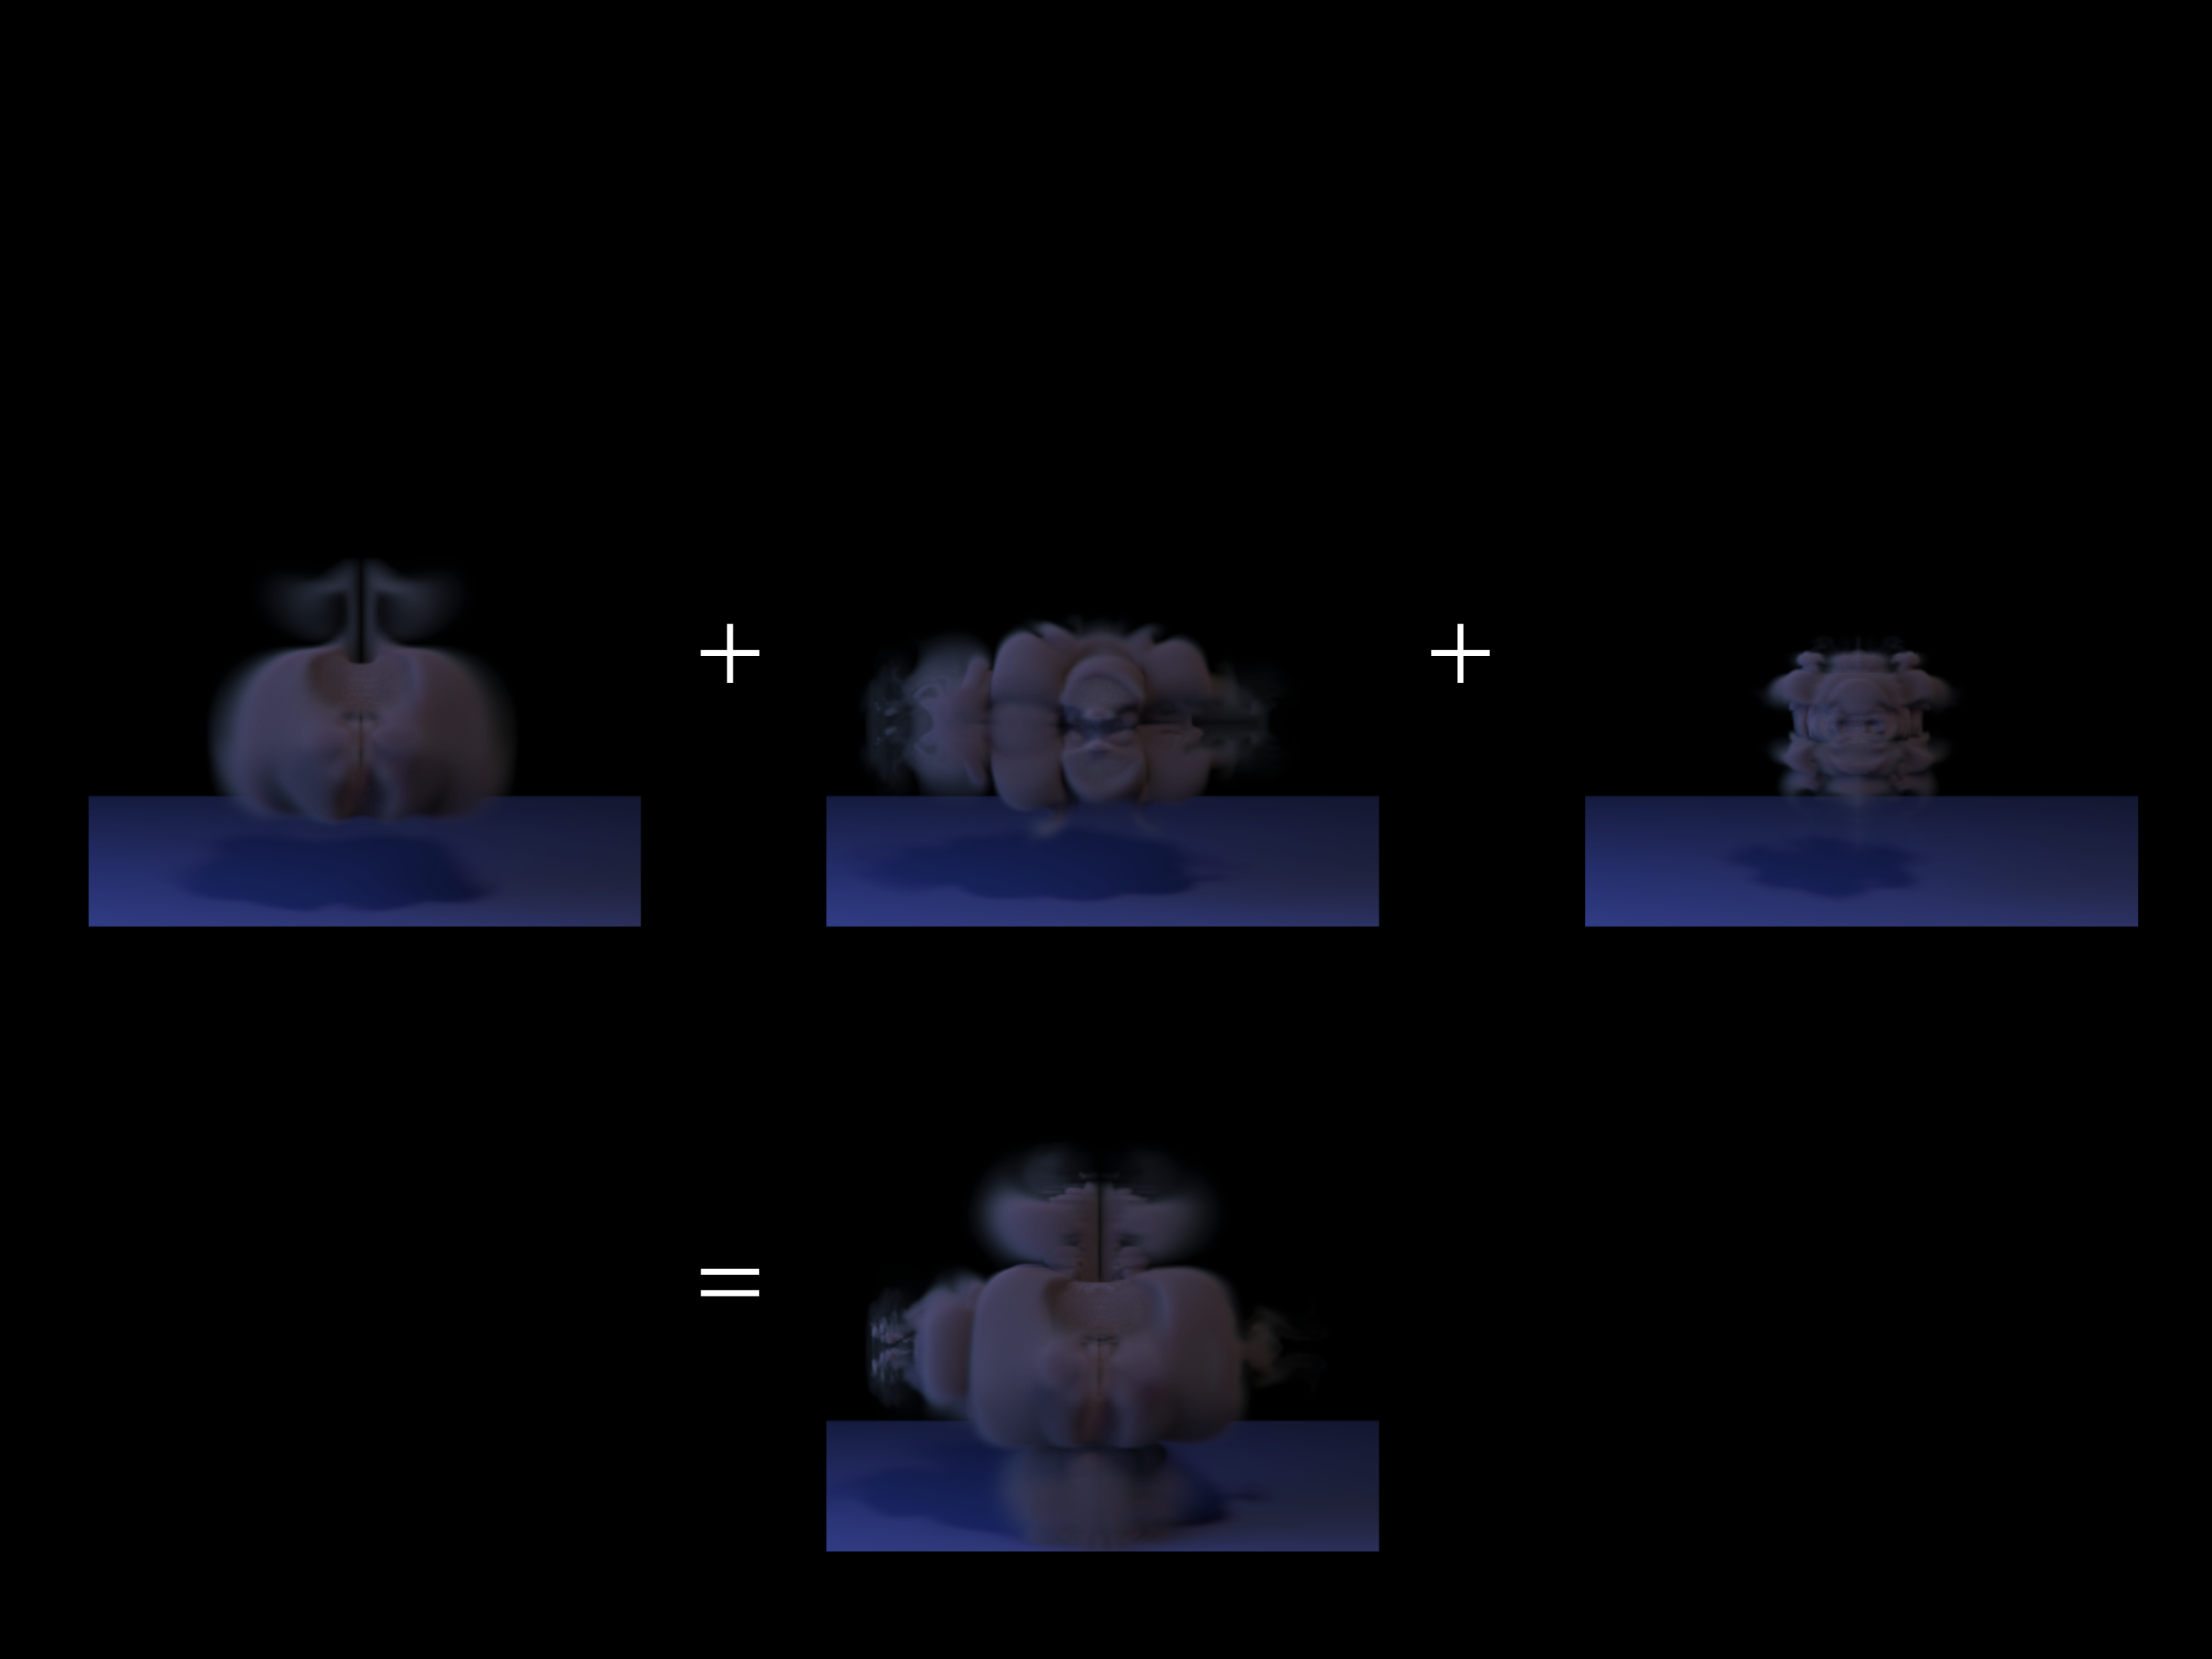
\includegraphics[width=\textwidth]{chap6/figures/superposition.png}
	\caption{Three individual modes in superposition produce a mixed modal shape.}
\label{fig:superposition}
\end{figure}

\section{Dynamic Control}
If we define the {\em energy} of a fluid snapshot in time as the $L_2$ norm of the vector of modal weights, then we see that as time unfolds, the energy waxes and wanes according to the strength
of the various modal weights. Accordingly, the sound increases or decreases in overall spectral density and loudness based on the same principle. However, by forgoing the physics-based time-evolution,
we can harness direct spectral control over the visuals and sound, producing simple and pleasing audiovisual gestures such as crescendo, diminuendi, and swells.

\begin{figure}
	\centering
	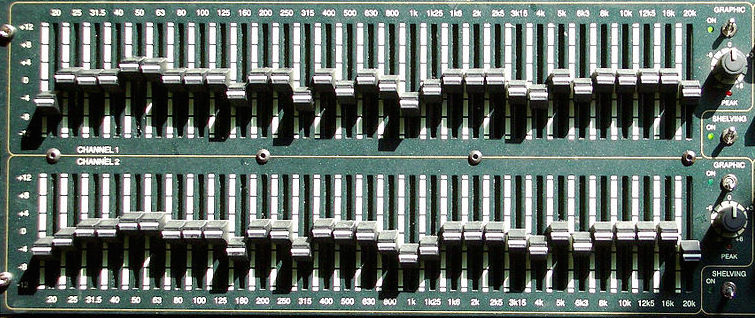
\includegraphics[width=\textwidth]{chap6/figures/faders.jpg}
	\caption{Each of the $r = 150$ modes can be controlled individually, analogous to a set of equalization faders. Source: Wikimedia Commons.}
\label{fig:faders}
\end{figure}

\begin{figure}
	\centering
	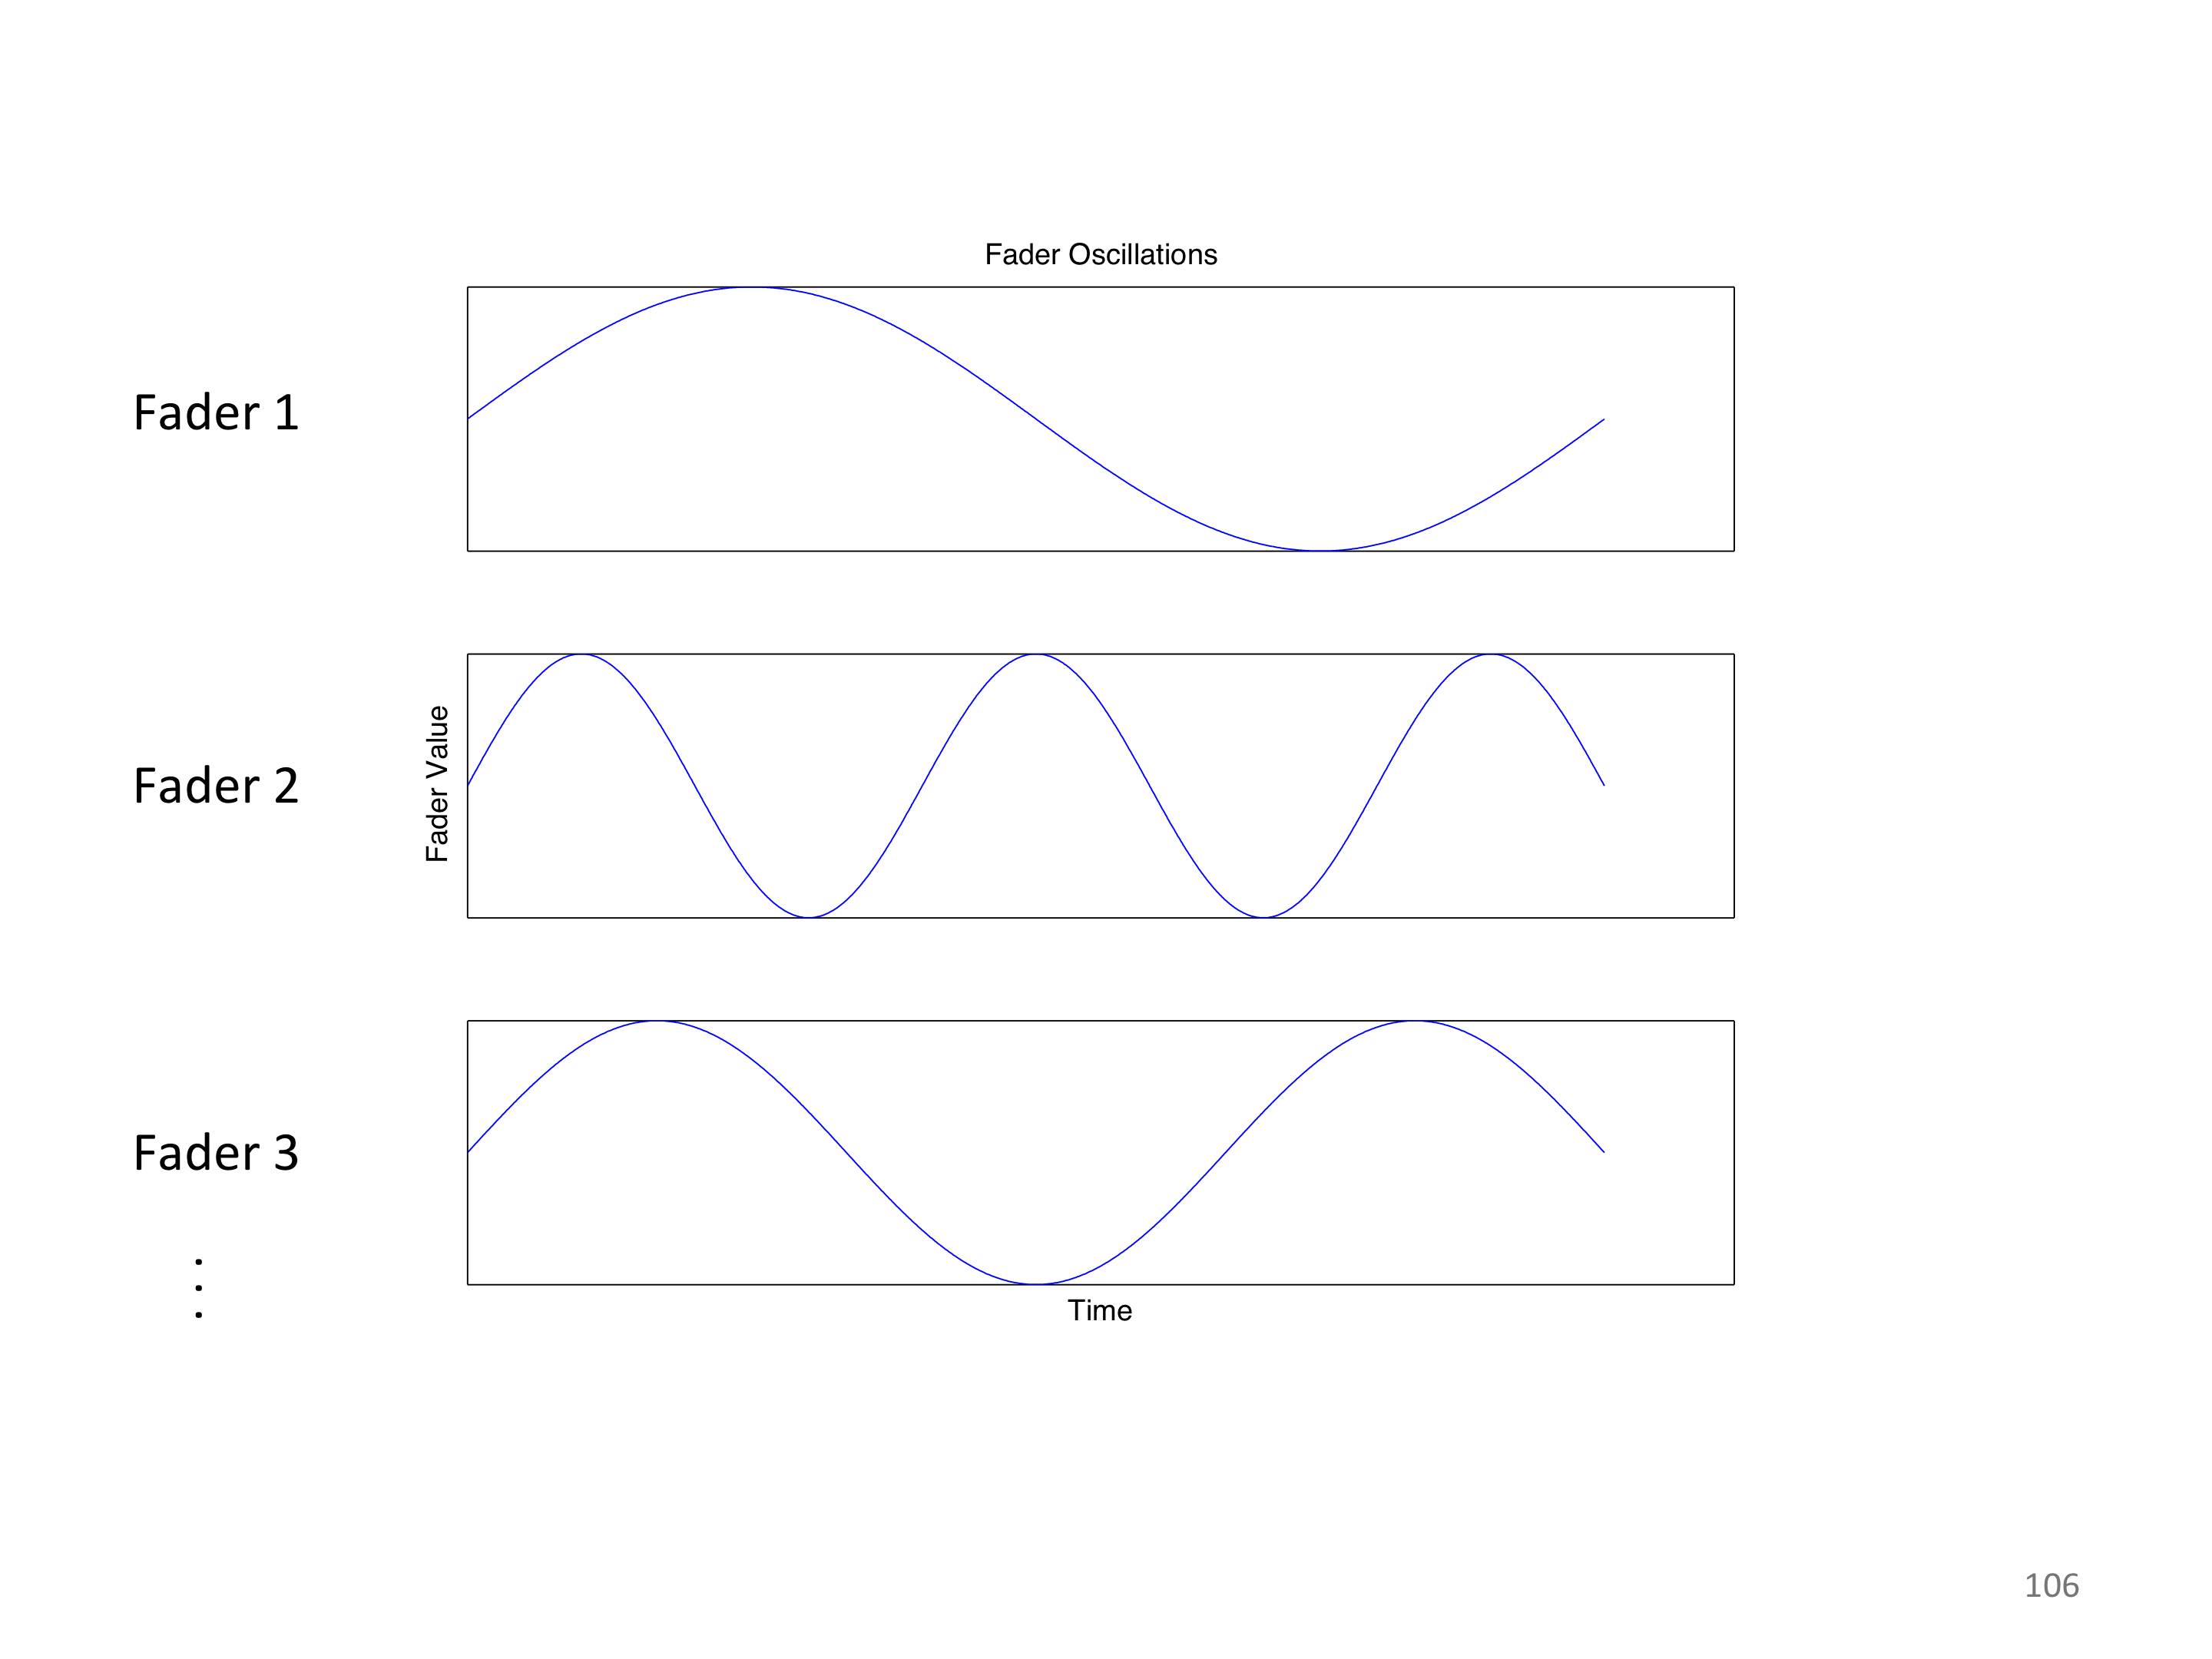
\includegraphics[width=\textwidth]{chap6/figures/fader_envelopes.png}
	\caption{Each modes's fader knob can be modulated smoothly over time, creating spectrally-varying envelopes.}
\label{fig:fader_envs}
\end{figure}



